\documentclass{cours}

\title{Convexité}

\begin{document}
    \maketitle{14}

    \begin{Gpartie}{Fonction Convexe et Fonction Concave} 
        \begin{Spartie}{Définitions} 
            Soit $f$ une fonction dérivable sur un intervalle $I$ et $\mathcal{C}$ sa courbe représentative dans un repère.

            $f$ est \emph{convexe} sur $I$ si quels que soient les points $A$ et $B$ de la courbe $\mathcal{C}$ sur $I$, le segment $\big[AB\big]$ est au dessus de $\mathcal{C}$ entre $A$ et $B$.

            $f$ est \emph{concave} sur $I$ si quels que soient les points $A$ et $B$ de la courbe $\mathcal{C}$ sur $I$, le segment $\big[AB\big]$ est en dessous de $\mathcal{C}$ entre $A$ et $B$.

            \begin{center}
                \begin{tikzpicture}
                    \begin{axis}[
                        xmin=-2, xmax=2,
                        ymin=-2, ymax=2,
                        xtick=\empty,
                        ytick=\empty
                    ]
                        \node[anchor=north west] at (0,-1.5) {$\mathcal{C}_f$};
                        \addplot[blue, very thick, samples=50, smooth]{x^2-1.5};
                        \node[dot, label=left:$A$] (A) at (-1,-0.5) {};
                        \node[dot, label=right:$B$] (B) at (1.5,0.75) {};
                        \draw[red, thick] (A) -- (B);
                    \end{axis}
                \end{tikzpicture}
                \hspace{1cm}
                \begin{tikzpicture}
                    \begin{axis}[
                        xmin=-2, xmax=2,
                        ymin=-2, ymax=2,
                        xtick=\empty,
                        ytick=\empty
                    ]
                        \addplot[blue, very thick, samples=50, smooth]{-x^2+1.5};
                        \node[anchor=south east] at (0,1.5) {$\mathcal{C}_f$};
                        \node[dot, label=left:$A$] (A) at (-1.5,-0.75) {};
                        \node[dot, label=right:$B$] (B) at (1,0.5) {};
                        \draw[red, thick] (A) -- (B);
                    \end{axis}
                \end{tikzpicture}
                \parbox{\linewidth}{\captionof{figure}{\centering Illustration de la Définition}}
            \end{center}
        \end{Spartie}
        \begin{Spartie}{Propriété} 
            Si $f$ est convexe sur $I$, pour tous réels $a$ et $b$ de $I$, $f\left(\frac{a+b}{2}\right)\leq\frac{f(a)+f(b)}{2}$.

            Si $f$ est concave sur $I$, pour tous réels $a$ et $b$ de $I$, $f\left(\frac{a+b}{2}\right)\geq\frac{f(a)+f(b)}{2}$.
            \begin{SSpartie}{Démonstration} 
                Supposons $f$ convexe.

                Soit $A~\left(a~;f(a)\right)$ et $B~\left(b~;f(b)\right)$ deux points de $\mathcal{C}$, alors $\big[AB\big]$ est au dessus de $\mathcal{C}$, en particulier, le milieu de $\big[AB\big]$ d'abscisse $\frac{a+b}{2}$ et d'ordonnée $\frac{f(a)+f(b)}{2}$ est au dessus de l'image de $\frac{a+b}{2}$ par $f$.
            \end{SSpartie}
        \end{Spartie}
        \begin{Spartie}{Propriété (admise)} 
            $f$ est convexe sur $I$ si et seulement si $\mathcal{C}$ est située au dessus de chacune de ses tangentes sur $I$

            $f$ est concave sur $I$ si et seulement si $\mathcal{C}$ est située en dessous de chacune de ses tangentes sur $I$

            \begin{center}
                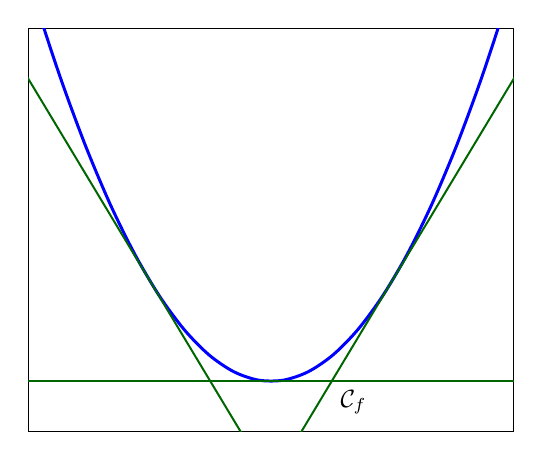
\begin{tikzpicture}[scale=0.9]
                    \begin{axis}[
                        xmin=-2, xmax=2,
                        ymin=-2, ymax=2,
                        xtick=\empty,
                        ytick=\empty
                    ]
                        \addplot[blue, very thick, samples=50, smooth]{x^2-1.5};
                        \addplot[black!60!green, thick]{-2*\x-2.5};
                        \addplot[black!60!green, thick]{-1.5};
                        \addplot[black!60!green, thick]{2*\x-2.5};
                        \node[anchor=north west] at (0.5,-1.5) {$\mathcal{C}_f$};

                    \end{axis}
                \end{tikzpicture}
                \hspace{1cm}
                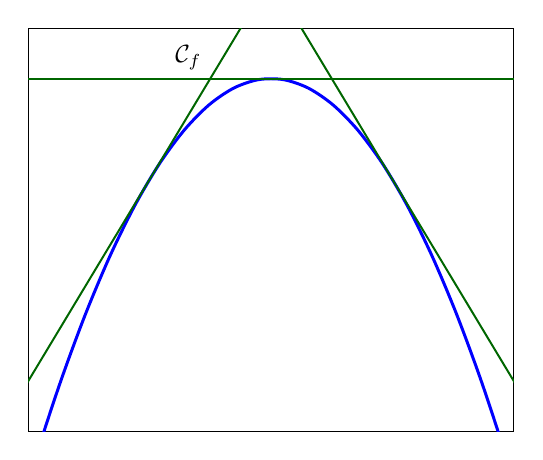
\begin{tikzpicture}[scale=0.9]
                    \begin{axis}[
                        xmin=-2, xmax=2,
                        ymin=-2, ymax=2,
                        xtick=\empty,
                        ytick=\empty
                    ]
                        \addplot[blue, very thick, samples=50, smooth]{-x^2+1.5};
                        \addplot[black!60!green, thick]{2*\x+2.5};
                        \addplot[black!60!green, thick]{-2*\x+2.5};
                        \addplot[black!60!green, thick]{1.5};
                        \node[anchor=south east] at (-0.5,1.5) {$\mathcal{C}_f$};
                    \end{axis}
                \end{tikzpicture}
                \parbox{\linewidth}{\captionof{figure}{\centering Illustration de la Propriété}}
            \end{center}
        \end{Spartie}
        \begin{Spartie}{Définition} 
            $A$ est un point d'inflexion de $\mathcal{C}$ si au point $A$, la courbe traverse sa tangente.

            \begin{center}
                \begin{tikzpicture}
                    \begin{axis}[
                        xmin=-3.25, xmax=3.25,
                        ymin=-4.25, ymax=4.25
                    ]
                        \addplot[blue, very thick, samples=50, smooth]{0.5*\x^3-1.5*\x};
                        \addplot[black!60!green, thick]{-1.5*\x};
                        \node[dot] at (0,0) {};
                        \node[anchor=south west] at (0,0) {$A$};
                    \end{axis}
                \end{tikzpicture}
                \parbox{\linewidth}{\captionof{figure}{\centering Exemple d'un Point d'Inflexion}}
            \end{center}
        \end{Spartie}
        \begin{Spartie}{Remarque} 
            Lorsque $f$ change de convexité, sa courbe $\mathcal{C}$ admet un point d'inflexion.
        \end{Spartie}
    \end{Gpartie}
    \pagebreak
    \begin{Gpartie}{Lien avec la Dérivée} 
        \begin{Spartie}{Définition} 
            Soit $f$ une fonction dérivable sur $I$ dont la fonction dérivée $f'$ est dérivable sur $I$. La dérivée de $f'$ se nomme la dérivée seconde de $f$ et se note $f''$.
        \end{Spartie}
        \begin{Spartie}{Propriété} 
            Soit $f$ une fonction dérivable deux fois sur un intervalle $I$.

            $f$ est convexe sur $I$ si et seulement si :
            \begin{itemize}
                \item $f'$ est croissante sur $I$
                \item $f''$ est positive sur $I$
                \item La courbe représentative est située au dessus de ses tangentes sur $I$
            \end{itemize}
        \end{Spartie}
        \begin{Spartie}{Propriété} 
            $f$ est concave sur $I$ si et seulement si :
            \begin{itemize}
                \item $f'$ est décroissante sur $I$
                \item $f''$ est négative sur $I$
                \item La courbe représentative est située en dessous de ses tangentes sur $I$
            \end{itemize}
        \end{Spartie}
        \begin{Spartie}{Propriété} 
            Si $\mathcal{C}$ est la courbe représentative de $f$ dans un repère, $\mathcal{C}$ admet un point d'inflexion au point d'abscisse $a$ si et seulement si $f''$ s'annule et change de signe en $a$.

            \begin{center}
                \begin{tikzpicture}
                    \begin{axis}[
                        xmin=-5.25, xmax=5.25,
                        ymin=-4.25, ymax=4.25,
                        legend pos=south east
                    ]
                        \addplot[blue, very thick, samples=50, smooth]{0.5*\x^3-1.5*\x};
                        \addplot[red, thick, samples=50, smooth]{1.5*\x^2-1.5};
                        \addplot[orange, thick, samples=50, smooth]{3*\x};
                        \addlegendentry{$f(x)$}
                        \addlegendentry{$f'(x)$}
                        \addlegendentry{$f''(x)$}
                        \node[dot] at (0,0) {};
                        \node[anchor=south west] at (0,0) {$A$};
                    \end{axis}
                \end{tikzpicture}
                \parbox{\linewidth}{\captionof{figure}{\centering Illustration de l'Évolution de la Convexité en Fonction de la Dérivée Seconde}}
            \end{center}
        \end{Spartie}
    \end{Gpartie}
\end{document}